

\chapter{INTRODUÇÃO}
\l{T}odo o ambiente é gratuito e todo o conteúdo deste livro está associado às tecnologias descritas neste tópico, qualquer outra tecnologia adicionada pelo aprendiz é de inteira responsabilidade destes, os links se encontram no próximo sub-tópico de acordo com a listagem, repare na nota de rodapé.

O computador do aprendiz deverá ter a capacidade de virtualização de sistemas operacionais 64 bits, geralmente os computadores já vem configurados para tal, mas se não for capaz, o aprendiz deve com as especificações de seu computador obter os manuais de configuração da BIOS e realizar a configuração manualmente.

\section{Tecnologias utilizadas e Download de arquivos}
Para iniciar, o aprendiz deve realizar o download dos seguintes artefatos:
\begin{itemize}
	\item VirtualBox para virtualizar as práticas, nunca realize as práticas diretamente no sistema operacional que utiliza diariamente;
	\item Debian versão 12 64bits Terminal para operar as práticas que são todas em GNU/Linux, mantenha esta versão para manter a coerência com as práticas;
	\item Putty e WinSCP para acessar remotamente as máquinas virtuais caso queira usar recurso CTRL+C e CTRL+V;
\end{itemize}



\section{Instalando o VirtualBox}
Se o aluno realizar as práticas em seu Sistema Operacional de uso diário, ou seja, se já é usuário GNU/Linux e queria fazer diretamente, este encontrará inúmeros problemas, pois as práticas afetam o sistema operacional. Para isso utilizamos uma camada de abstração, ou seja, uma camada de virtualizarão, será utilizado para fins de padronização o VirtualBox da Oracle. Conforme Figura \ref{fig:linux1}.

\begin{figure}[h]
	\centering
	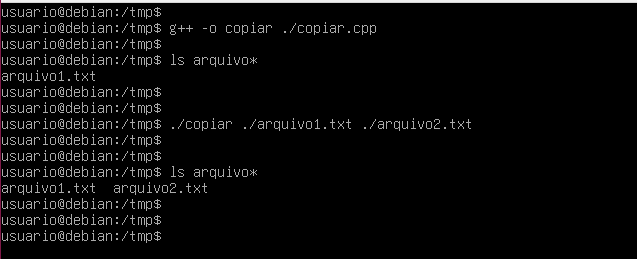
\includegraphics[width=0.6\textwidth]{cap/introducao/figure/linux.png}
	\caption{a Uma figura qualquer}
	\label{fig:linux1}
\end{figure}


